\documentclass{ieeeaccess}

% --- Packages ---
\usepackage{cite}
\usepackage{amsmath,amssymb,amsfonts}
\usepackage{algorithmic}
\usepackage{graphicx}
\usepackage{textcomp}
\usepackage{caption}
\usepackage{mathptmx}
\usepackage{hyperref}
\usepackage[english]{babel}
\usepackage{microtype}
\usepackage{xurl}
\usepackage{bm}
\usepackage{booktabs}
\usepackage{array}
\usepackage[section]{placeins}
\usepackage{dblfloatfix}

% --- Float spacing tweaks ---
\setlength{\textfloatsep}{10pt plus 2pt minus 2pt}
\setlength{\floatsep}{8pt plus 2pt minus 2pt}
\setlength{\intextsep}{8pt plus 2pt minus 2pt}

% --- Bold math setup ---
\makeatletter
\AtBeginDocument{\DeclareMathVersion{bold}
\SetSymbolFont{operators}{bold}{T1}{times}{b}{n}
\SetSymbolFont{NewLetters}{bold}{T1}{times}{b}{it}
\SetMathAlphabet{\mathrm}{bold}{T1}{times}{b}{n}
\SetMathAlphabet{\mathit}{bold}{T1}{times}{b}{it}
\SetMathAlphabet{\mathbf}{bold}{T1}{times}{b}{n}
\SetMathAlphabet{\mathtt}{bold}{OT1}{pcr}{b}{n}
\SetSymbolFont{symbols}{bold}{OMS}{cmsy}{b}{n}
\renewcommand\boldmath{\@nomath\boldmath\mathversion{bold}}}
\makeatother

\def\BibTeX{{\rm B\kern-.05em{\sc i\kern-.025em b}\kern-.08em
    T\kern-.1667em\lower.7ex\hbox{E}\kern-.125emX}}

\newcommand{\tracebox}[1]{%
\noindent\fbox{%
\begin{minipage}{0.96\columnwidth}
\ttfamily\footnotesize
#1
\end{minipage}}}

\begin{document}

\history{Date of publication xxxx 00, 0000, date of current version xxxx 00, 0000.}
\doi{xx.xxxx/ACCESS.xxxx.xxxxxxx}

\title{Multi-Agent AgentGym-RL: Collapse Onset, Recovery, and Prevention in BabyAI and WebArena Multi-Turn RL}
\author{\uppercase{Mavino Ikein}}
\address{Georgia Institute of Technology, Atlanta, GA, USA (e-mail: mikein3@gatech.edu)}
\corresp{Corresponding author: Mavino Ikein (e-mail: mikein3@gatech.edu).}

\markboth
{Ikein: Multi-Agent AgentGym-RL Collapse Across BabyAI and WebArena}
{Ikein: Multi-Agent AgentGym-RL Collapse Across BabyAI and WebArena}

\begin{abstract}
Single-agent multi-turn RL can substantially improve long-horizon LLM agents, but many deployed systems rely on \emph{multi-agent} role decomposition such as planner--executor pipelines. We study what happens when those role-separated systems are trained end-to-end with multi-turn RL, focusing on three concrete questions: \emph{when does collapse begin, can the run recover once instability appears, and what evidence suggests how collapse might be prevented?} We analyze six cooperative multi-agent regimes across BabyAI and WebArena: tagged two-agent ScalingInter-RL, fixed-round no-tag two-agent training, two no-tag ScalingInter-RL curricula, a three-agent planner--executor--reviewer extension, and a clean two-agent WebArena transfer. In BabyAI, no-tag ScalingInter-RL reaches strong intermediate checkpoints that exceed the single-agent baseline (best two-agent checkpoint: Pass@1 $=0.8222$ at step $300$), but all long runs eventually collapse. Tagged prompts induce an early scaffold-copying failure; no-tag runs remove that specific mode but still suffer late executor-side or interface-wide collapse. The three-agent reviewer changes the failure mode and permits partial recovery after early instability, but still reaches full collapse by step $450$. In WebArena, collapse can begin almost immediately: traces show a grounded planner at step $1$, warning signs by step $2$, and a fully collapsed sampled batch by step $9$, while every saved checkpoint from $50$ through $600$ evaluates to zero success. The combined evidence shows that multi-agent training instability is regime-dependent, partial recovery is possible only before full collapse, and late-stage failure is best understood as a protocol/interface problem rather than a simple monotonic decline in reward.
\end{abstract}

\begin{keywords}
LLM agents, multi-agent reinforcement learning, multi-turn RL, long-horizon tasks, training stability, collapse analysis, AgentGym-RL, BabyAI, WebArena, prompt design.
\end{keywords}

\titlepgskip=-21pt
\maketitle

\section{Introduction}
Multi-turn LLM agents must repeatedly observe an environment, propose an action, receive feedback, and continue until success or failure. Long-horizon tasks are difficult because early mistakes compound, recovery becomes harder, and small distribution shifts can destabilize learned behavior. AgentGym-RL showed that reinforcement learning can improve \textbf{single-agent} multi-turn performance by optimizing end-to-end task completion under a structured training loop and a progressive interaction-horizon curriculum \cite{agentgymrl2025}.

At the same time, many practical agent systems are already \textbf{multi-agent}: a planner produces an intent and an executor carries out a concrete action. This decomposition is attractive because it mirrors how deployed agent stacks are often built. However, it is not well understood whether cooperative multi-agent role separation remains stable when trained end-to-end with multi-turn RL over long horizons.

This paper asks three concrete questions:
\begin{enumerate}
\item \textbf{When does collapse begin?}
\item \textbf{Can the system recover after instability starts?}
\item \textbf{What evidence suggests how collapse might be prevented?}
\end{enumerate}

We answer these questions with checkpoint metrics, trace packets, and cross-run comparisons across BabyAI and WebArena. The main result is not that multi-agent training is uniformly better; instead, the strongest defensible story is that multi-agent decomposition can produce strong intermediate checkpoints, but the training process exhibits \textbf{multiple distinct collapse modes}. Those modes depend on prompt regime, topology, and environment. Tagged prompts induce early scaffold-copying collapse, no-tag BabyAI runs push collapse later into the executor or role interface, a reviewer introduces a new schema-contamination route, and WebArena shows that collapse is not BabyAI-specific and can begin almost immediately.

\section{Related Work}
\textbf{Multi-turn RL for LLM agents.} AgentGym-RL established a training recipe that treats LLM agent behavior as sequential decision-making and optimizes task completion using multi-turn RL \cite{agentgymrl2025}. Our work inherits its training/evaluation structure and uses its single-agent BabyAI result as the primary baseline.

\textbf{Cooperative MARL baselines.} Cooperative MARL has developed methods to stabilize shared-reward teams, including centralized-training paradigms and value-decomposition approaches \cite{maddpg2017,qmix2018,mappo2021}. These ideas motivate careful curricula and instrumentation, but language policies introduce additional failure channels such as format violations, scaffold copying, schema leakage, and prompt drift.

\textbf{Multi-agent LLM orchestration.} Systems such as AutoGen, MetaGPT, and CAMEL demonstrate that role specialization via prompting can improve collaborative performance without RL \cite{autogen2023,metagpt2023,camel2023}. Our setting differs because the roles are trained under RL pressure; this makes prompt artifacts themselves part of the learned behavior.

\textbf{Long-horizon benchmarks.} BabyAI provides a tightly controlled instruction-following testbed, while WebArena introduces higher-entropy browser interaction and a stricter action contract \cite{babyai2018,webarena2023,scienceworld2022,agentbench2023}. We use BabyAI to diagnose collapse mechanisms and WebArena to test whether those mechanisms generalize.

\section{Experimental Setup}
\subsection{A. Environments and role topologies}
Our primary development environment is \textbf{BabyAI} \cite{babyai2018}, selected because it provides multi-step interaction, a strict action format, sparse success, and highly auditable traces. We extend the analysis to \textbf{WebArena} \cite{webarena2023} as a cross-environment stress test.

We study the following role topologies:
\begin{itemize}
\item \textbf{Two-agent planner--executor}: the planner emits language guidance and the executor emits the environment-facing action.
\item \textbf{Three-agent planner--executor--reviewer}: the reviewer inspects the executor output and can request a retry or pass.
\end{itemize}

All runs optimize a shared team reward. In the baseline experiments analyzed here, the roles share one underlying policy and differ only through prompts and turn structure.

\subsection{B. Regimes}
We analyze six primary regimes:
\begin{enumerate}
\item \textbf{Tagged two-agent ScalingInter-RL}: planner/executor prompts include visible role tags.
\item \textbf{Fixed-round two-agent no-tag}: visible role tags removed, no horizon scaling.
\item \textbf{Two-agent no-tag ScalingInter-RL, coarse schedule}: curriculum `[6,13,20]`.
\item \textbf{Two-agent no-tag ScalingInter-RL, dense schedule}: curriculum `[6,8,10,13,16,20]`.
\item \textbf{Three-agent no-tag ScalingInter-RL with executor reviewer}.
\item \textbf{WebArena clean two-agent no-tag ScalingInter-RL}: simplified planner--executor topology with the executor aligned to the original single-agent WebArena action contract.
\end{enumerate}

\subsection{C. Baseline and metrics}
For BabyAI we compare against the \textbf{single-agent AgentGym-RL baseline}:
\begin{itemize}
\item \textbf{Single-agent baseline:} Pass@1 $=0.7333$, Avg@1 $=0.6728$
\end{itemize}

We report:
\begin{itemize}
\item \textbf{Pass@1}
\item \textbf{Avg@1}
\item \textbf{ExecutorNativeFormatViolations}
\item \textbf{InvalidFormatTerminationRate}
\item \textbf{InvalidActionTerminationRate}
\item \textbf{PlannerInvalidFormatRate}
\item \textbf{PlannerFallbackRate}
\item \textbf{PlannerTagOnlyRate}
\end{itemize}

In addition, our trace analysis uses concrete packets from:
\begin{itemize}
\item `/Users/mavinomichael/PycharmProjects/AgentGym-RL/reports/2026-03-30_multi_agent_collapse_paper_handoff/selected_trace_packets.md`
\item `/Users/mavinomichael/PycharmProjects/AgentGym-RL/reports/2026-03-30_multi_agent_collapse_paper_handoff/collapse_regime_summary.tsv`
\end{itemize}

\section{Results}
\subsection{A. Unified regime summary}
Table~\ref{tab:regime_summary} summarizes the regimes in question-led form: peak checkpoint, first warning, full collapse, and whether recovery is observed before full collapse.

\begin{table*}[!t]
\centering
\caption{Unified regime summary with collapse timing and recovery. WebArena is included as cross-environment evidence rather than a directly comparable success benchmark.}
\label{tab:regime_summary}
\resizebox{\textwidth}{!}{%
\begin{tabular}{llcccccc}
\toprule
Environment & Regime & Peak Step & Peak Pass@1 & Peak Avg@1 & First Warning & Full Collapse & Recovery Before Full Collapse \\
\midrule
BabyAI & Single-agent baseline & 0 & 0.7333 & 0.6728 & --- & --- & --- \\
BabyAI & 2-agent tagged ScalingInter-RL & 50 & 0.8000 & 0.7443 & 55 & 100 & No \\
BabyAI & 2-agent fixed-round no-tag & 100 & 0.6778 & 0.6399 & 400 & 400 & No \\
BabyAI & 2-agent no-tag ScalingInter-RL `[6,13,20]` & 200 & 0.8111 & 0.7552 & 400 & 450 & No \\
BabyAI & 2-agent no-tag ScalingInter-RL `[6,8,10,13,16,20]` & 300 & 0.8222 & 0.7743 & 400 & 450 & No \\
BabyAI & 3-agent no-tag + reviewer & 100 & 0.7222 & 0.6918 & 150 & 450 & Yes, at 250--350 \\
WebArena & Clean 2-agent no-tag ScalingInter-RL & 50 & 0.0000 & 0.0000 & 2 & 9 & No \\
\bottomrule
\end{tabular}%
}
\end{table*}

The main quantitative pattern is:
\begin{enumerate}
\item \textbf{Intermediate gains are real in BabyAI.} The best two-agent no-tag checkpoints exceed the single-agent baseline.
\item \textbf{Those gains are not stable through the full horizon.} Every long BabyAI run eventually collapses.
\item \textbf{WebArena is harsher.} The collapse problem appears almost immediately and persists across the entire saved checkpoint frontier.
\end{enumerate}

\subsection{B. Success and failure curves}
Figure~\ref{fig:success_panels} compares the main BabyAI success curves. Figure~\ref{fig:failure_panels} shows the associated failure metrics. Figure~\ref{fig:collapse_questions_fig} adds two question-led views: collapse timing relative to the training horizon, and recovery before versus after early warning. Figure~\ref{fig:webarena_panels} shows the WebArena clean 2-agent collapse profile separately.

\begin{figure*}[!t]
\centering
\begin{minipage}[t]{0.48\textwidth}
\centering
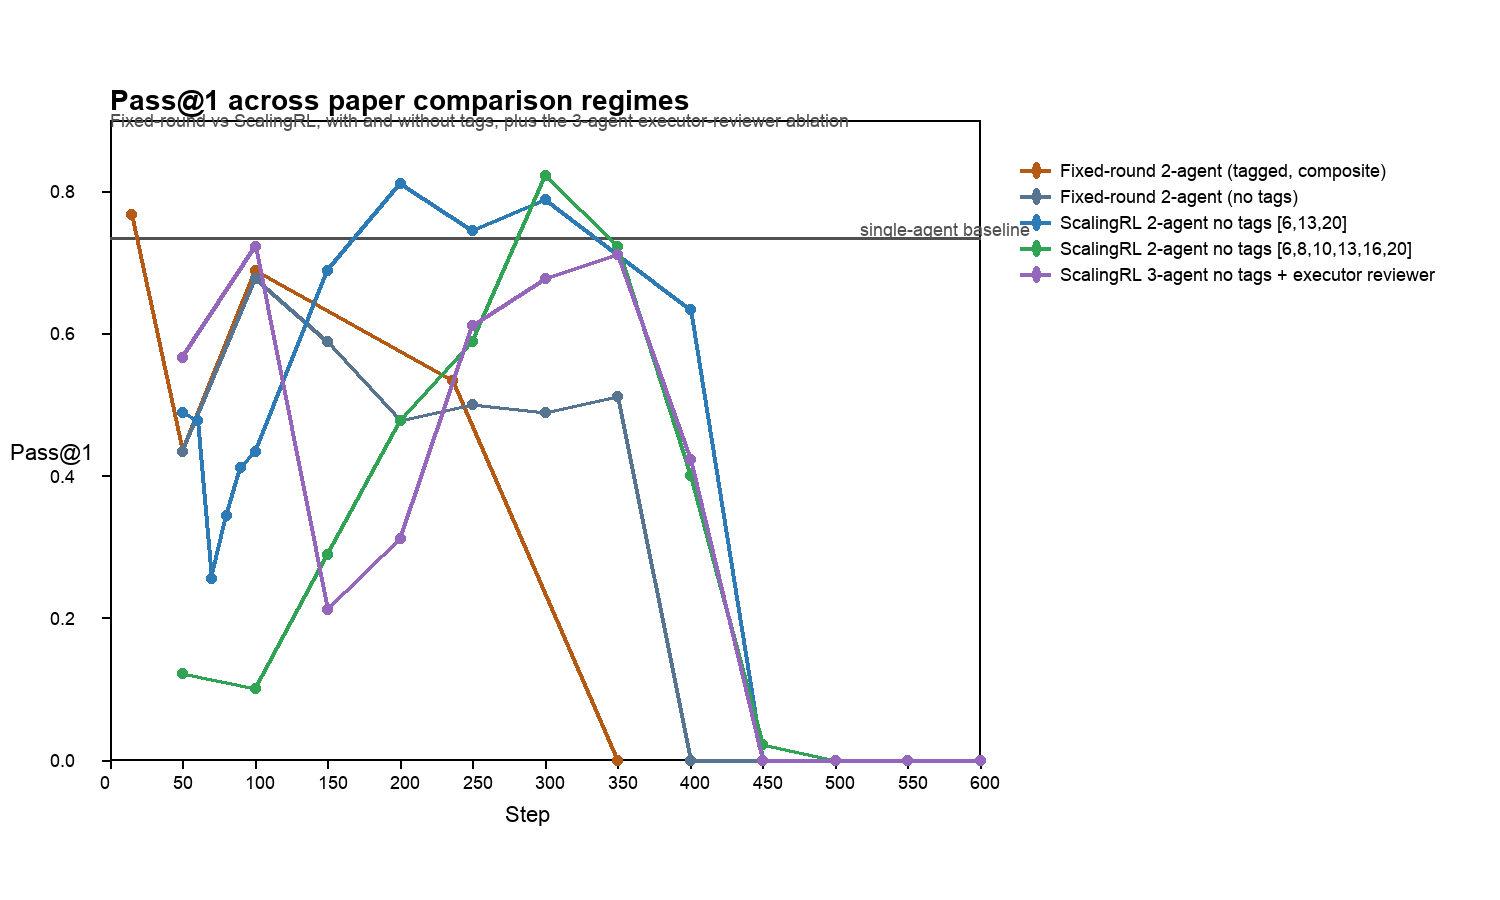
\includegraphics[width=\linewidth,height=0.25\textheight,keepaspectratio]{figures/fig_pass1_comparison.png}
\end{minipage}\hfill
\begin{minipage}[t]{0.48\textwidth}
\centering
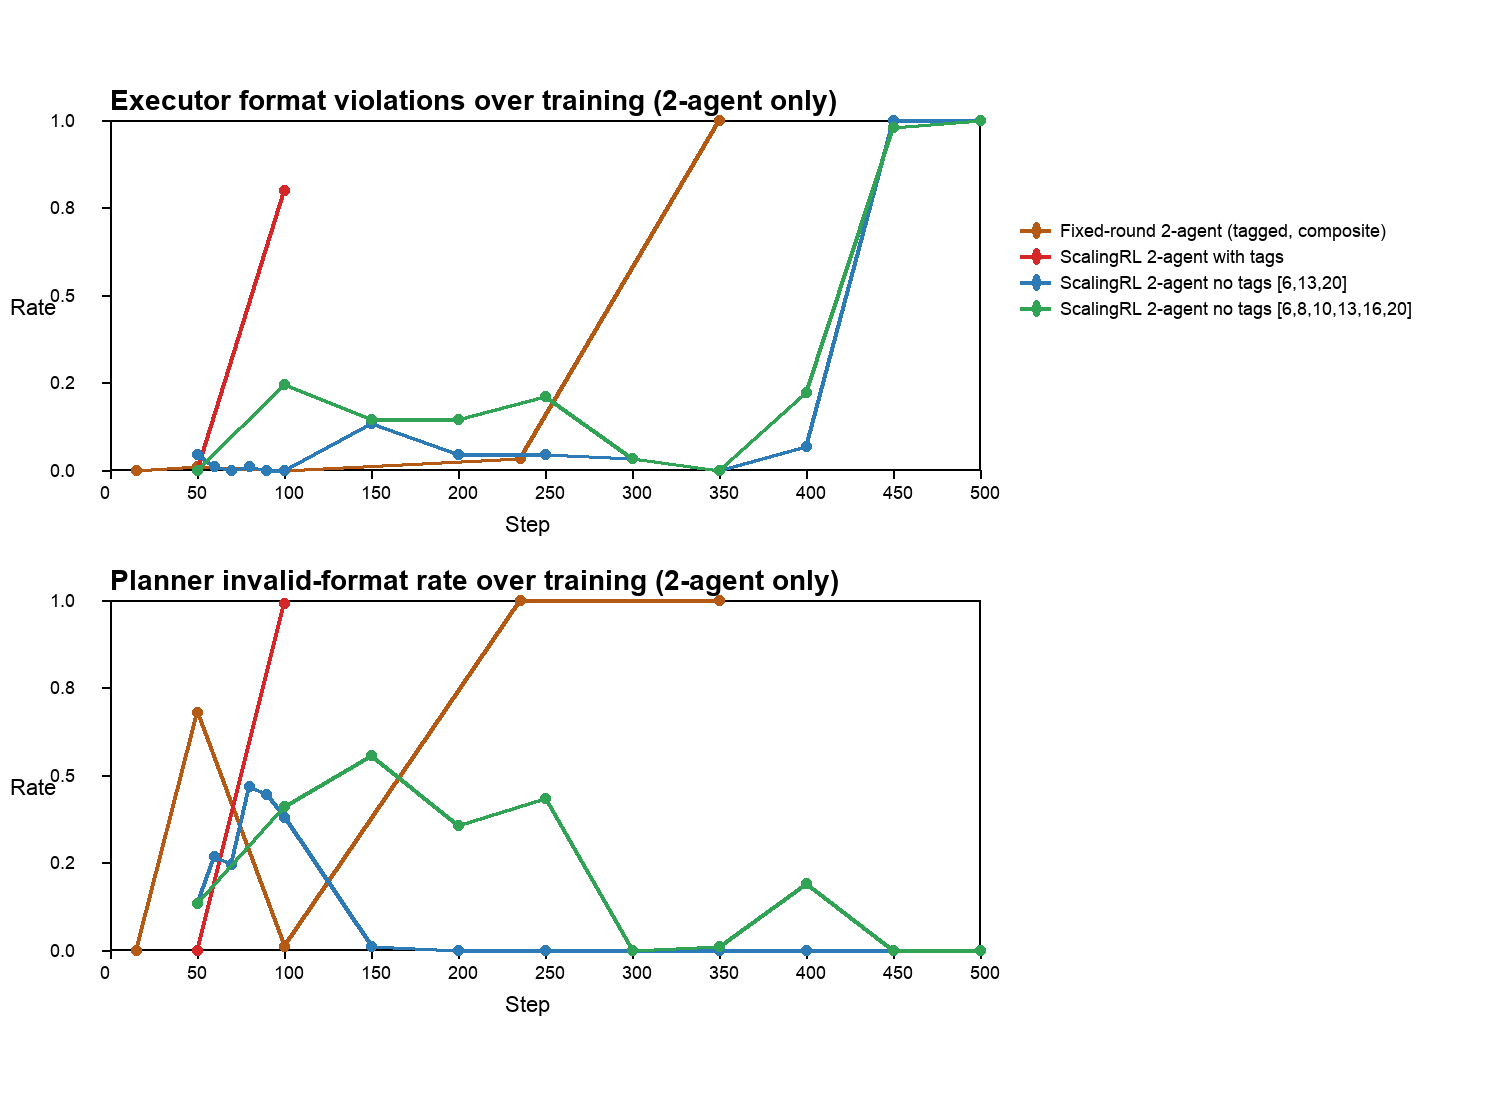
\includegraphics[width=\linewidth,height=0.25\textheight,keepaspectratio]{figures/fig_failure_comparison.png}
\end{minipage}
\caption{BabyAI regime comparison. Left: Pass@1 across major two-agent and three-agent regimes, with the single-agent baseline as reference. Right: executor and planner failure metrics across the same regimes.}
\label{fig:success_panels}
\end{figure*}

\begin{figure*}[!t]
\centering
\begin{minipage}[t]{0.48\textwidth}
\centering
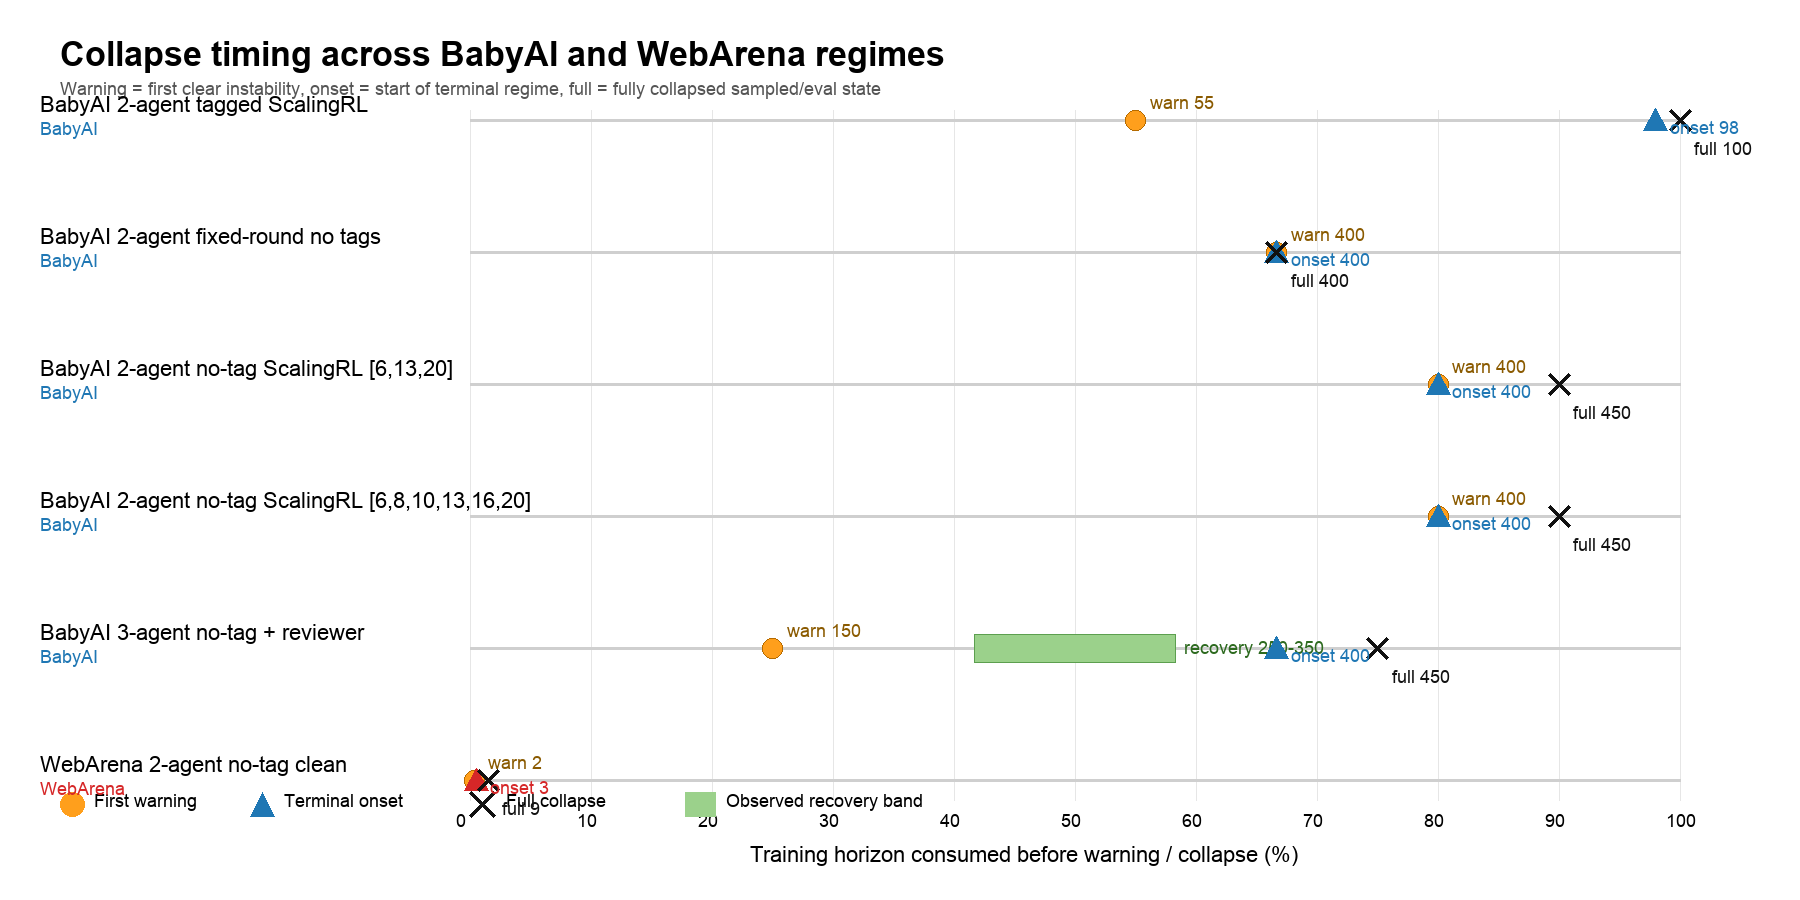
\includegraphics[width=\linewidth,height=0.24\textheight,keepaspectratio]{figures/fig_collapse_timeline.png}
\end{minipage}\hfill
\begin{minipage}[t]{0.48\textwidth}
\centering
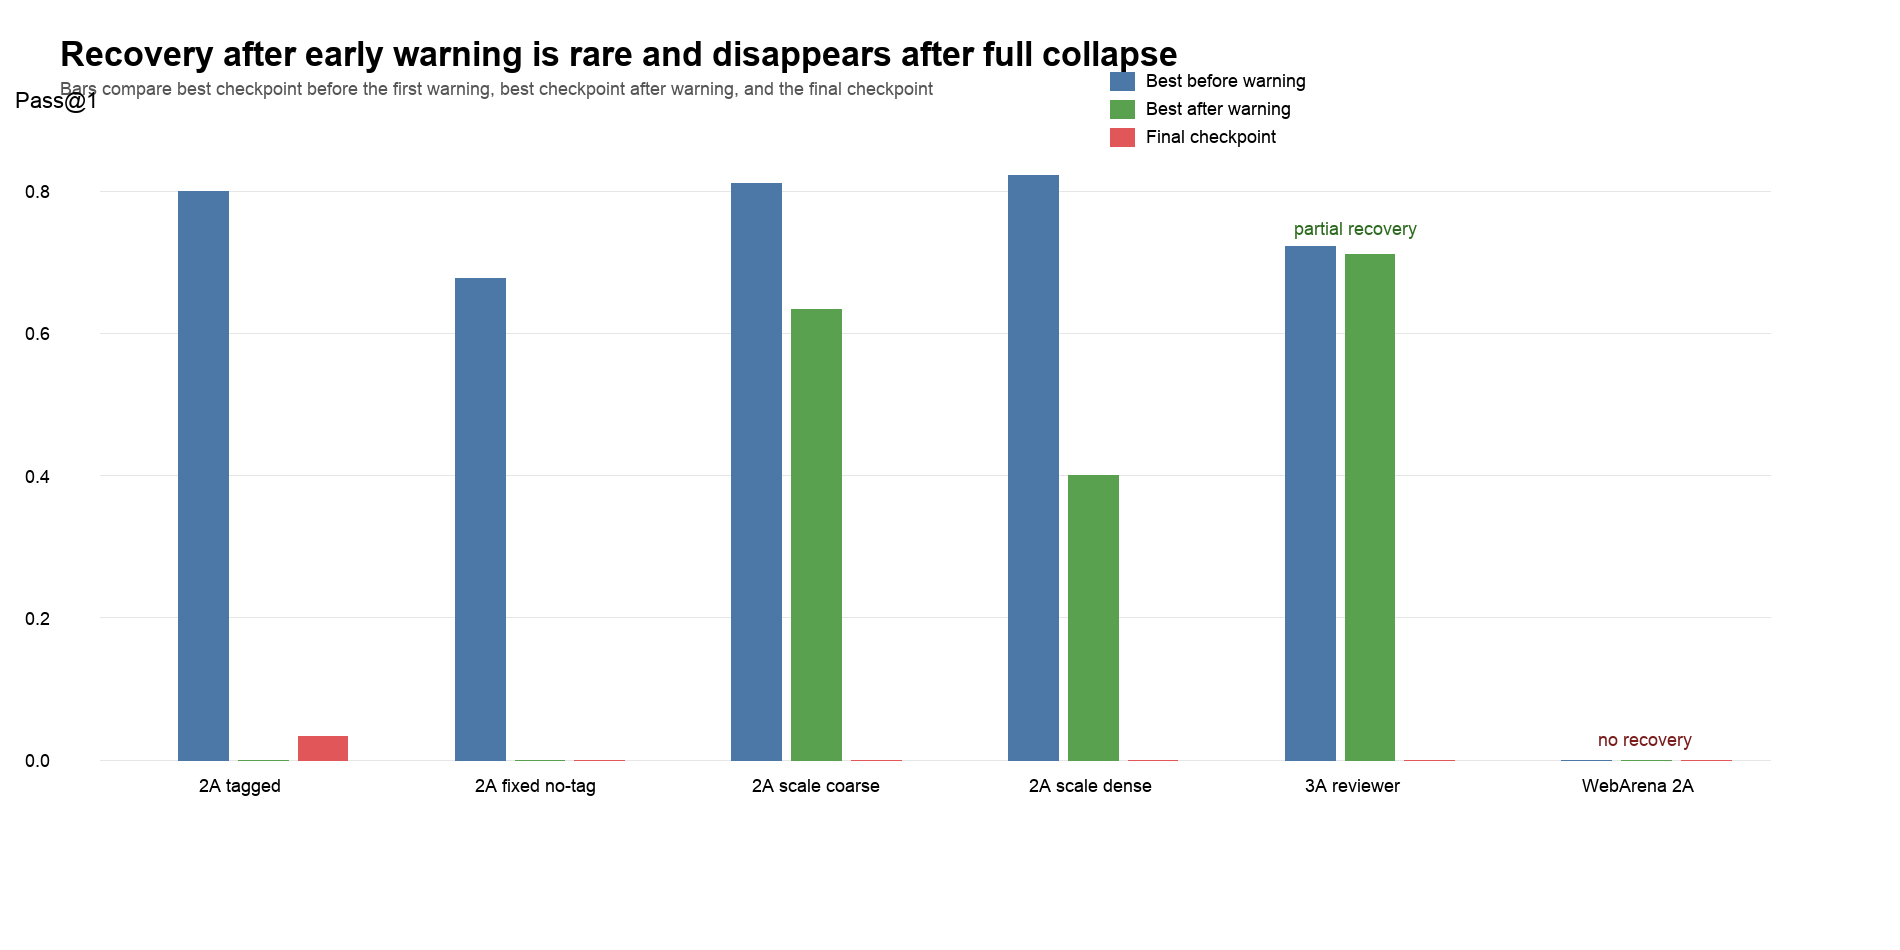
\includegraphics[width=\linewidth,height=0.24\textheight,keepaspectratio]{figures/fig_recovery_summary.png}
\end{minipage}
\caption{Question-led collapse views. Left: first warning, terminal onset, and full collapse normalized by training horizon. Right: best checkpoint before warning, best checkpoint after warning, and final checkpoint. The only clear recovery band is the 3-agent reviewer run at steps 250--350.}
\label{fig:collapse_questions_fig}
\end{figure*}

\begin{figure*}[!t]
\centering
\begin{minipage}[t]{0.48\textwidth}
\centering
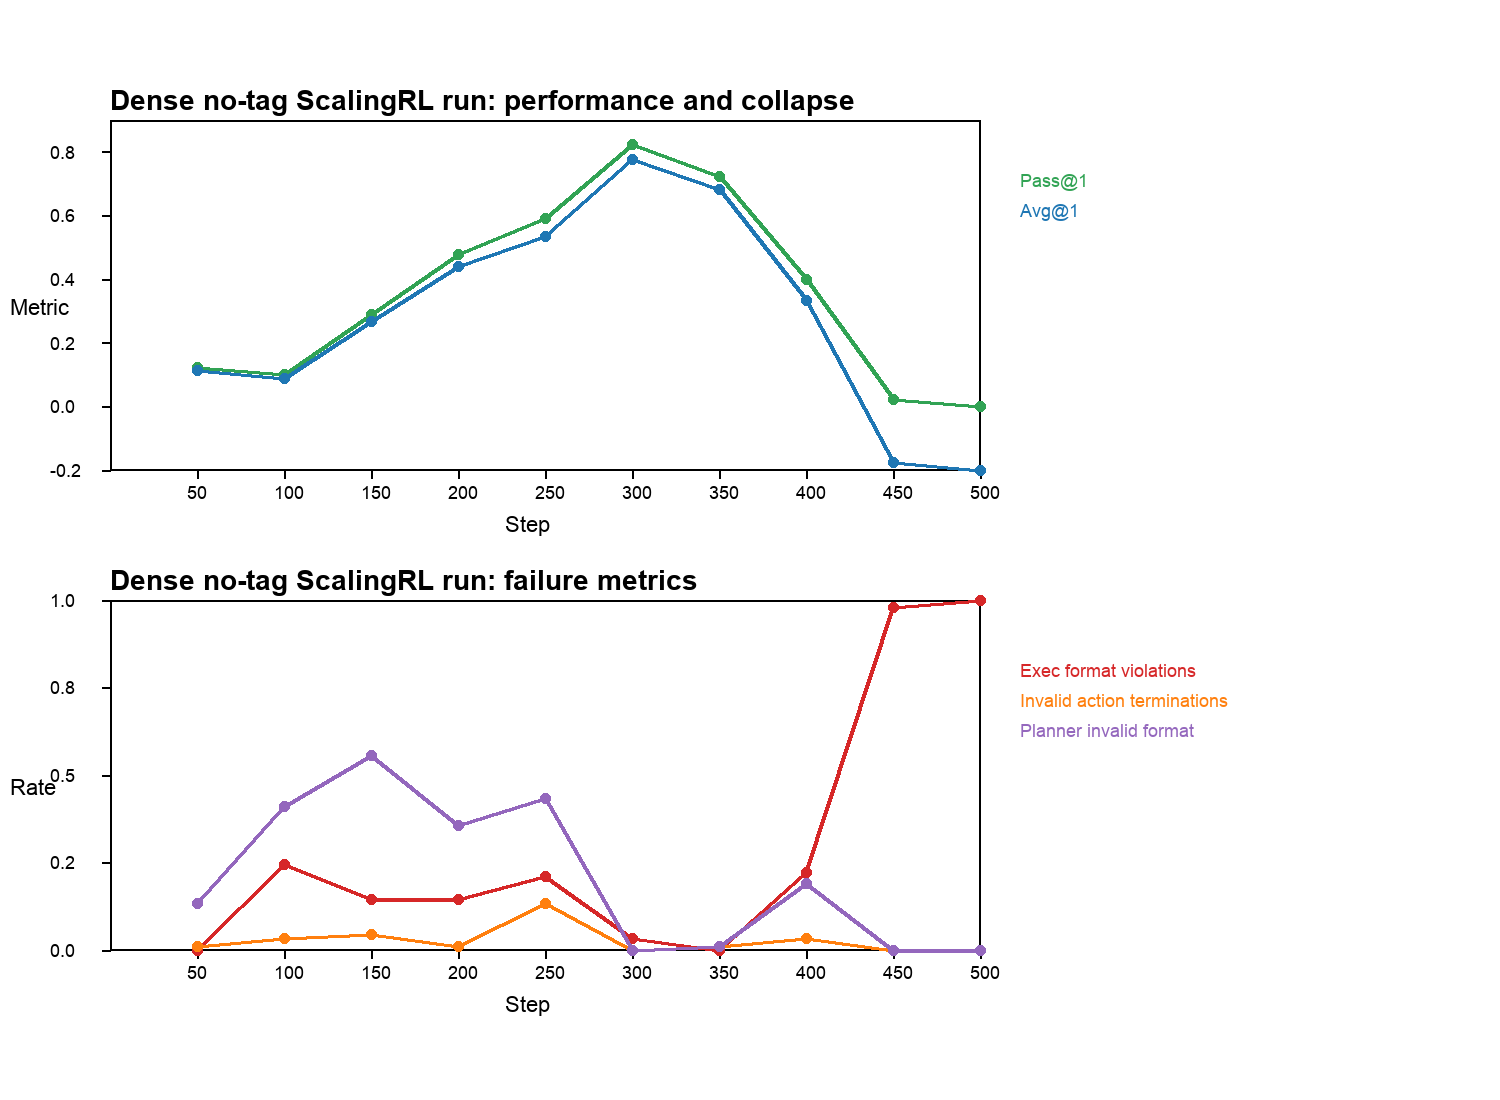
\includegraphics[width=\linewidth,height=0.25\textheight,keepaspectratio]{figures/fig_dense500_detail.png}
\end{minipage}\hfill
\begin{minipage}[t]{0.48\textwidth}
\centering
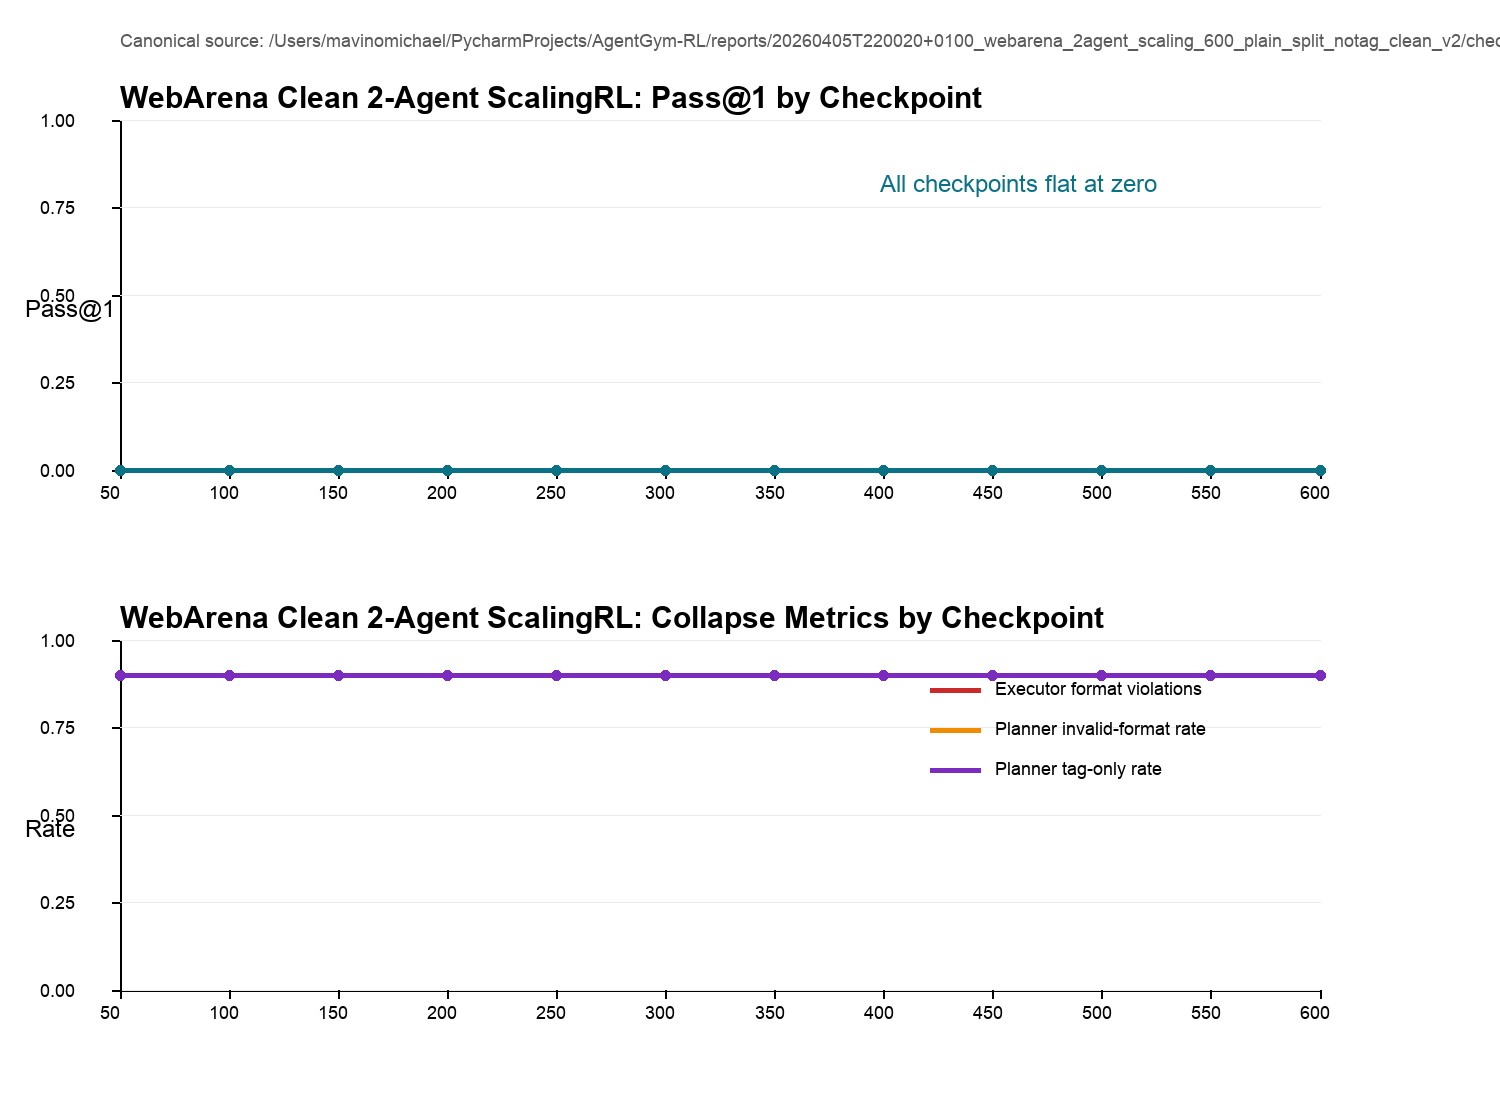
\includegraphics[width=\linewidth,height=0.25\textheight,keepaspectratio]{figures/fig_webarena_clean_v2_collapse.png}
\end{minipage}
\caption{Detailed views. Left: dense no-tag BabyAI ScalingInter-RL showing strong performance at step 300 and late executor collapse at 450--500. Right: WebArena clean 2-agent collapse, which never develops a stable evaluation frontier.}
\label{fig:webarena_panels}
\end{figure*}

\FloatBarrier

\section{Collapse Questions}
\subsection{A. When does collapse begin?}
Collapse onset is \textbf{not uniform}. It depends strongly on the regime.

\textbf{Tagged two-agent ScalingInter-RL.} Collapse begins early. The first visible warning appears by \textbf{step 55}, where the planner starts copying visible prompt headers into its plan. By \textbf{step 100}, the run reaches near-terminal recursive scaffold contamination: Pass@1 falls to $0.0333$, executor format violations rise to $0.8$, and planner invalid-format reaches $0.9889$.

\textbf{No-tag BabyAI ScalingInter-RL.} Collapse is later and more gradual. In the dense run, the system remains strong through \textbf{step 350}, degrades at \textbf{step 400}, and fully collapses by \textbf{450--500}. The coarse no-tag run shows the same pattern, with collapse arriving slightly earlier in terms of performance loss after the step-200 peak.

\textbf{Fixed-round no-tag BabyAI.} Collapse is late but abrupt. The run remains healthy through \textbf{step 350}, then flips into full failure at \textbf{step 400}, where Pass@1 becomes $0.0$ and both planner and executor invalid-format metrics saturate.

\textbf{Three-agent reviewer.} Collapse begins in two stages. The first instability arrives at \textbf{step 150}, where reviewer-schema failures and false retries cause a sharp performance drop. The terminal collapse begins at \textbf{step 400} and becomes complete by \textbf{step 450}.

\textbf{WebArena clean two-agent.} Collapse begins almost immediately. The only clearly healthy trace is at \textbf{step 1}. Warning signs appear by \textbf{step 2}, the first concrete tag-only failure appears at \textbf{step 3}, and the first fully collapsed sampled batch appears by \textbf{step 9}. Every saved checkpoint from \textbf{50} through \textbf{600} evaluates to zero success.

\subsection{B. Is collapse sudden or gradual?}
The answer is \textbf{regime-specific}.
\begin{itemize}
\item \textbf{Gradual}: dense and coarse no-tag ScalingInter-RL show a strong mid-run region, then a transition band, then full collapse.
\item \textbf{Sudden}: fixed-round no-tag BabyAI flips from healthy at step 350 to full collapse at step 400.
\item \textbf{Near-immediate}: WebArena collapses before the first saved checkpoint.
\end{itemize}

\subsection{C. Can the system recover after instability starts?}
Only \textbf{partially}, and only before full collapse.

The clearest recovery evidence is the \textbf{3-agent reviewer} run. It drops badly at steps \textbf{150--200}, then recovers to Pass@1 values of \textbf{0.6111}, \textbf{0.6778}, and \textbf{0.7111} at steps \textbf{250}, \textbf{300}, and \textbf{350}. This shows that an unstable run is not necessarily doomed immediately.

However, once a run reaches \textbf{full collapse}, we do \textbf{not} observe spontaneous recovery in any regime. Tagged two-agent, dense no-tag two-agent, coarse no-tag two-agent, fixed-round no-tag two-agent, and WebArena all remain collapsed after their terminal transition.

\subsection{D. Does adding more agents help, or just create new failure modes?}
Adding a reviewer does \textbf{not} solve collapse. It changes the failure mode.

The three-agent reviewer run never exceeds the best two-agent dense no-tag checkpoint. Its best checkpoint is \textbf{step 100} with Pass@1 $=0.7222$, below the two-agent dense best of \textbf{0.8222} at step 300. What the reviewer adds is not a higher peak, but a \textbf{recovery band} after early instability. The cost is a new interface failure surface: reviewer-schema contamination of executor outputs and malformed reviewer pass/retry decisions.

\subsection{E. Is collapse planner-driven, executor-driven, or interface-driven?}
The answer differs by regime:
\begin{itemize}
\item \textbf{Tagged two-agent}: planner-driven scaffold leakage that contaminates the executor.
\item \textbf{Dense no-tag two-agent}: late collapse is primarily executor-side; planner remains formally valid while executor format failure saturates.
\item \textbf{Three-agent reviewer}: interface-driven early, then full three-channel contamination later.
\item \textbf{WebArena clean two-agent}: planner tag-only collapse appears almost immediately, then executor invalid-format termination dominates.
\end{itemize}

Across the runs, the most defensible summary is that collapse is often an \textbf{interface instability}: one role degrades first, but the failure becomes system-wide when protocol structure starts leaking or breaking across channels.

\subsection{F. Is collapse environment-specific, or does it generalize beyond BabyAI?}
It clearly \textbf{generalizes beyond BabyAI}. WebArena shows the same core problem in a harsher form: protocol collapse can happen almost immediately and remain flat-zero across the full eval frontier.

This matters because it weakens the claim that BabyAI collapse is only a narrow artifact of a gridworld action space. The evidence suggests the deeper problem is not just the environment, but the fragility of the role interface under RL.

\subsection{G. Does removing tags help?}
\textbf{Yes, but only partially.}

Removing visible role tags removes the specific \emph{header-copying} failure mode seen in the tagged regime. It also unlocks the strongest intermediate checkpoints in BabyAI. But tag removal alone does not prevent:
\begin{itemize}
\item fixed-round no-tag total collapse at step 400,
\item late dense/coarse no-tag executor collapse at 450--500,
\item near-immediate WebArena collapse.
\end{itemize}

\subsection{H. Once full collapse happens, does the model recover later?}
In the observed runs, \textbf{no}. There is no evidence of recovery after the model reaches a full-collapse regime where invalid-format metrics saturate and success drops to zero.

\section{Collapse Taxonomy with Trace Examples}
\subsection{A. Tagged scaffold-copying collapse}
In the tagged regime, visible prompt headers become learnable tokens. The planner begins to emit prompt scaffolding directly, and the executor copies that scaffold instead of producing a valid environment action.

\subsection{B. No-tag late executor collapse}
Removing tags eliminates the header-copying mode and enables strong intermediate checkpoints, but late in training the executor becomes the strict bottleneck. In the dense run at step 450, executor format violations reach $0.9778$ while planner invalid-format remains at $0.0$.

\subsection{C. Reviewer schema interference collapse}
The reviewer introduces a new failure surface. At step 150 it already produces malformed schema; by step 350 reviewer text leaks into executor output; by step 450 planner, executor, and reviewer are all degenerate.

\subsection{D. WebArena near-immediate planner tag-only collapse}
The clean WebArena run removes reviewer complexity and aligns the executor to the single-agent action contract, yet still collapses almost immediately. The dominant trace signature is planner tag-only or punctuation garbage followed by executor invalid-format termination.

\begin{figure*}[!t]
\centering
\begin{minipage}[t]{0.48\textwidth}
\textbf{Tagged scaffold collapse}\\[4pt]
\tracebox{Planner: [Planner Turn] Move right to the red ball [Executor Turn]\\
Executor: [Executor Turn] Move right to the red ball [Planner Turn]}
\end{minipage}\hfill
\begin{minipage}[t]{0.48\textwidth}
\textbf{Late no-tag executor degradation}\\[4pt]
\tracebox{Planner: Move right to get the ball.\\
Executor: turn left.}
\end{minipage}

\vspace{8pt}

\begin{minipage}[t]{0.48\textwidth}
\textbf{Reviewer schema leakage}\\[4pt]
\tracebox{Executor: Thought: pick up the key\\
Action: pickup yellow key 1\\
Verdict: PASS\\
Reason: Valid format}
\end{minipage}\hfill
\begin{minipage}[t]{0.48\textwidth}
\textbf{WebArena tag-only collapse}\\[4pt]
\tracebox{Planner: !!!!!!!!!!!!!!!!!!!!!!!!!!!!!!!!\\
Executor: !!!!!!!!!!!!!!!!!!!!!!!!!!!!!!!!\\
Env: Terminated due to invalid executor output (invalid\_format)}
\end{minipage}
\caption{Representative trace patterns for the main collapse modes. These excerpts are shortened from the trace packets in `/Users/mavinomichael/PycharmProjects/AgentGym-RL/reports/2026-03-30_multi_agent_collapse_paper_handoff/selected_trace_packets.md`.}
\label{fig:trace_examples}
\end{figure*}

\FloatBarrier

\section{Discussion}
\subsection{A. What the evidence directly supports}
Our data support five strong conclusions:
\begin{enumerate}
\item collapse onset is regime-dependent;
\item partial recovery is possible before terminal collapse, but only in some regimes;
\item full collapse is not observed to recover later;
\item removing tags removes one failure mode but does not stabilize training overall;
\item the collapse problem is not BabyAI-specific.
\end{enumerate}

\subsection{B. Interpretive mechanisms suggested by the traces}
Three explanations are especially consistent with the evidence.

\textbf{First, free-form planner text leaks scaffolding into downstream roles.} This is directly visible in the tagged BabyAI run, in the 3-agent reviewer schema leak, and in WebArena tag-only planner collapse. The common theme is that when planner text is unconstrained, it can become a high-salience source of non-environment-native tokens that the executor later copies.

\textbf{Second, shared reward likely blurs credit assignment across roles.} In the dense no-tag BabyAI run, the planner remains formally valid while the executor collapses late. Yet both roles are optimized under the same team-level signal. This makes it plausible that the executor can be ``dragged'' by a learning signal that does not cleanly isolate its format failures.

\textbf{Third, planner and executor likely should not be treated as a homogeneous PPO population.} The planner emits free-form guidance, while the executor must satisfy a strict action contract. Their error distributions and reward interfaces differ. Our experiments did not directly ablate role-wise normalization or role-specific credit assignment, so we do \emph{not} claim causality here; however, the observed executor-dominant late collapse is consistent with that mechanism.

\subsection{C. What seems most promising for prevention}
Our experiments do not provide a complete prevention recipe, but they do suggest a practical hierarchy:
\begin{itemize}
\item remove visible prompt scaffolding;
\item monitor format metrics as early-stop signals;
\item select checkpoints near the last stable band instead of training blindly to the horizon;
\item treat reviewer-schema leakage and planner tag-only outputs as explicit collapse warnings;
\item harden the planner--executor contract so that planner text is less able to contaminate executor actions.
\end{itemize}

\section{Limitations}
This study emphasizes collapse diagnosis rather than a fully stabilized training recipe. The fixed-round tagged evidence pool is partly composite rather than a single uninterrupted run. WebArena is represented by one clean two-agent run rather than a full ablation grid. Finally, some explanatory claims in the discussion are best interpreted as \emph{trace-consistent hypotheses} rather than isolated causal ablations.

\section{Conclusion}
This paper reframed multi-agent AgentGym-RL as a collapse investigation rather than a simple improvement story. In BabyAI, no-tag ScalingInter-RL can produce strong intermediate checkpoints that exceed the single-agent baseline, but every long multi-agent run eventually collapses. Tagged prompts induce early scaffold-copying failure, reviewer-based training introduces a new schema-interference route, and WebArena shows that collapse is not BabyAI-specific and can begin almost immediately. The most important practical lesson is that collapse is best analyzed as a role-interface problem with identifiable warning signs, not as a mysterious late-stage reward drop alone.

\FloatBarrier
\clearpage

\nocite{agentgymrl2025,babyai2018,webarena2023,scienceworld2022,agentbench2023}
\nocite{maddpg2017,qmix2018,mappo2021,autogen2023,metagpt2023,camel2023}

\bibliographystyle{IEEEtran}
\bibliography{references}

\EOD
\end{document}
